\section{Base Model}
First, we set out to develop a base model. However, first, we had to decide which image size to use. We choose an image size of 224x224, as this size seems to capture enough details, see page Appendix B - 0.5 Image Size. Also, many of the pretrained models uses the same image size, making our model more comparable to these. Resizing the images has the effect of making training of the model significantly faster and less focused on finer details.

Next, we had to decide how many layers our model should have. As the task is relatively simple, we decided to use 4 convolutional layers and 3 fully connected layers, including the binary output layer. Since the input images are in color and 224x224 pixels, inputting that image directly into the fully connected layers would result in a $224 \cdot 224 \cdot 3 = 150528$ input size into the model. We would like to reduce this further, so the fully connected layers does not get an input of 150528. The convolution layers extract features, which makes it possible for the neural network to recognise a specific feature no matter where it is in the image, instead of having to learn that feature for every possible position in an image.

For the loss function, we choose the cross-entropy since it is generally good and popular for classification tasks. For the optimizer, we choose Adam as it combines the strength of several other optimizers. Since we have 4/5 convolutional layers we choose to go with a pretty small kernel size of 3 by 3. A small kernel size is good for preserving details and since we have several convolutional layers it is still possible for us to capture broader features. We use max pooling after each convolutional layer for several reasons. First of all it improves generalization since it focuses on more prominent features. It reduces the dimensionality of the layer, which mean less computation and also reducing complexity so overfitting is less likely. For the activation function, we choose ReLU, as it is the most used activation function for convolutional neural networks.

Note that the architecture of the model is highly configurable making it easy to experiment with different configurations like different layers, kernels and regularization, see Appendix A - convolutionalNetwork.py. 

The final base model is provided in Table \ref{tab:base_model}.
\begin{table}[H]
    \vspace*{-0.5cm}
    \centering
    \begin{tabular}{|l|c|c|c|c|}
    \hline
                & \textbf{Output}           & \textbf{Kernel}   & \textbf{MaxPooling}   & \textbf{Activation}   \\ 
                & \textbf{kernels/features} &                   &   &   \\ \hline
    Conv2D w/   & 32                        & 3x3                   & 2x2                   & ReLU                  \\ \hline
    Conv2D w/   & 64                        & 3x3                   & 2x2                   & ReLU                  \\ \hline
    Conv2D w/   & 128                       & 3x3                   & 2x2                   & ReLU                  \\ \hline
    Conv2D w/   & 256                       & 3x3                   & 2x2                   & ReLU                  \\ \hline
    Linear w/   & 256                       & -                     & -                     & ReLU                  \\ \hline
    Linear w/   & 128                       & -                     & -                     & ReLU                  \\ \hline
    Linear w/   & 2                         & -                     & -                     & -                     \\ \hline
    \end{tabular}
    \caption{Base Model.}
    \label{tab:base_model}
    \vspace*{-0.8cm}
\end{table}

The model was trained for 25 epochs as a start. The learning rate was set to 0.001 as this is a generally good choice. A learning rate that is too small could result in a very slow learning process that might get stuck, and a too big learning rate could result in a local minimum or an unstable learning process. Results of the base model after 25 epochs are shown in Figure \ref{fig:base_model_results}.
\begin{figure}[H]
    \vspace*{-0.7cm}
    \centering
    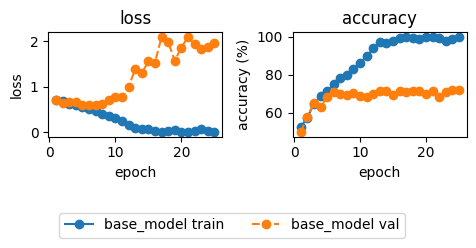
\includegraphics[width=0.4\textwidth]{figures/results_base_model.png}
    \caption{Base Model Results.}
    \label{fig:base_model_results}
    \vspace*{-0.7cm}
\end{figure}

Clearly, the base model is overfitting, therefore, we need to add some regularization to the model.